\documentclass[12pt]{article}
\usepackage{graphicx} % Required for inserting images
\usepackage{enumitem}
\usepackage{mathtools}
\usepackage{amsmath}
\usepackage{gvv-book}
\usepackage{gvv}

\title{\textbf{4.13.9}}
\author{\textbf{EE25BTECH11004 - Aditya Appana}}
\date{September 20, 2025}

\begin{document}

\maketitle

\section*{Question}
Let the algebraic sum of the perpendicular distances from the points (2,0),(0,2) and
(1,1) to a variable straight line be zero; then the line passes through a fixed point
whose coordinates are \rule{1.5cm}{0.15mm}.

\section*{Solution}

The normal form of a line is:
\begin{align}
\vec{n}^T\vec{x} = c
\end{align}\\
The perpendicular distance of a point from a line is:
\begin{align}
\frac{|\vec{n}^T\vec{x} - c|}{||n||}
\end{align}\\
It is given that the algebraic sum of the perpendicular distances of three points (2,0), (0,2), and (1,1) to a line $\vec{n}^T\vec{x} = c$ is 0. Therefore:

\begin{align}
\frac{\vec{n}^Tx_1 - c}{||n||} + \frac{\vec{n}^T\vec{x}_2 - c}{||n||} + \frac{\vec{n}^T\vec{x}_3 - c}{||n||} = 0
\end{align}\\

\begin{align}
\frac{\vec{n}^T(\vec{x}_1 +\vec{x}_2+ \vec{x}_3)- 3c}{||n||} = 0
\end{align}
So, the required point is:

\begin{align}
\frac{(\vec{x}_1 +\vec{x}_2+ \vec{x}_3)}{3}
\end{align}

Substituting the points:

\begin{align}
\frac{\myvec{2\\0} + \myvec{0\\2} + \myvec{1\\1} }{3} =\\
\myvec{1\\1}
\end{align}\\
Therefore the line passes through the fixed point (1,1).

\begin{figure}[H]
    \centering
    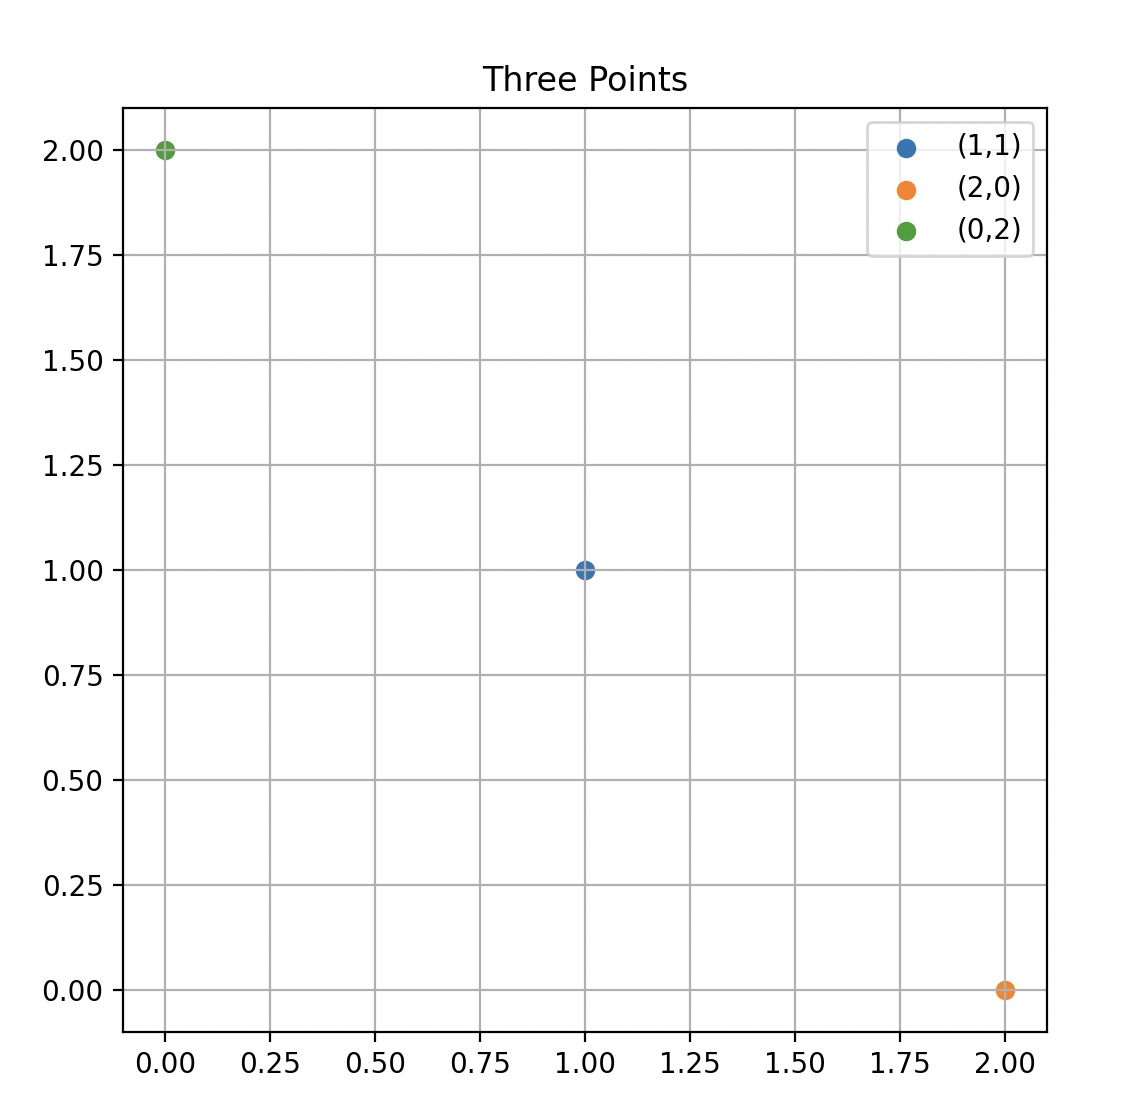
\includegraphics[width=0.7\columnwidth]{Figs/527.png}
    \caption{Plot}
    \label{fig:placeholder}
\end{figure}



\end{document}